
\de{ĐỀ THI HỌC KỲ I NĂM HỌC 2022-2023}{THPT Chuyên Lê Quý Đôn - Ninh Thuận}
\begin{center}
	\textbf{PHẦN 1 - TRẮC NGHIỆM}
\end{center}
\Opensolutionfile{ans}[ans/ans]


\begin{ex}%[10_HK1_LEQUYDON-NINHTHUAN_TL_TN]%[VU Ngoc Hao]%[0D3Y2-2]
	Cho hàm số bậc hai $y=ax^2+bx+c,(a\ne 0)$ có bảng biến thiên như hình dưới. Hàm số nghịch biến trên khoảng nào sau đây?
\begin{center}
	
\begin{tikzpicture}
		\tkzTabInit[nocadre=false,lgt=1.2,espcl=2.5,deltacl=0.6]
		{$x$ /0.6,$y$ /2}
		{$-\infty$,$-2$,$+\infty$}
		\tkzTabVar{+/$+\infty$,-/$-1$,+/$+\infty$}
	\end{tikzpicture}
\end{center}
	\choice
	{$(-\infty;0)$}
	{$(-2;+\infty )$}
	{\True $(-\infty;-2)$}
	{$(-\infty;-1)$}
	\loigiai{
	Từ bảng biến thiên suy ra hàm số nghịch biến trên khoảng $(-\infty;-2)$.


}
\end{ex}

\begin{ex}%[10_HK1_LEQUYDON-NINHTHUAN_TL_TN]%[VU Ngoc Hao]%[0D1Y3-2]
\immini{	Cho hai tập $A,B$ minh họa bằng biểu đồ Ven (như hình vẽ bên). Phần tô đậm trong hình là tập nào sau đây?
	\choice
	{$A\cup B$}
	{\True $A\setminus B$}
	{$A\cap B$}
	{$B\setminus A$}}{\begin{tikzpicture}[line join=round, line cap=round,>=stealth]
		\tikzset{label style/.style={font=\footnotesize}}
		\draw[pattern=north east 
		lines] (0,0) ellipse ({1.5} and {1});
		\draw[fill=white] (1.7,0) ellipse ({1.5} and {1});
		\draw (0,0) ellipse ({1.5} and {1});
		\fill[color=black] (-1,0) node[right] {$A$};
		\draw[color=black] (2.5,0) node[right] {$B$};
\end{tikzpicture}}
	\loigiai{
Hiệu của hai tập hợp $A$ và $B$ là tập gồm các phần tử thuộc $A$ nhưng không thuộc $B$. Kí hiệu $A\setminus B$.
}
\end{ex}

\begin{ex}%[10_HK1_LEQUYDON-NINHTHUAN_TL_TN]%[VU Ngoc Hao]%[0D2Y1-1]
	Cặp số $(x;y)$ nào sau đây {\bf không phải} là nghiệm của bất phương trình $3x-2y+1\ge 0$?
	\choice
	{\True $(0;1)$}
	{$(3;5)$}
	{$(1;0)$}
	{$(0;-1)$}
	\loigiai{
Ta có $3\cdot 0-2\cdot 1+1=-1<0$. Do đó cặp số $(x;y)=(0;1)$ không phải là nghiệm của bất phương trình đã cho.	
}
\end{ex}

\begin{ex}%[10_HK1_LEQUYDON-NINHTHUAN_TL_TN]%[VU Ngoc Hao]%[0H2Y1-2]
	Điều kiện cần và đủ để 3 điểm phân biệt $A,B,C$ thẳng hàng là
	\choice
	{ $\overrightarrow{AB}$ và $\overrightarrow{AC}$ cùng phương}
	{$\overrightarrow{AB}$ và $\overrightarrow{AC}$ cùng hướng}
	{\True $\overrightarrow{AB}$ và $\overrightarrow{AC}$ ngược hướng}
	{$\overrightarrow{AB}$ và $\overrightarrow{AC}$ là hai vectơ bằng nhau}
	\loigiai{
Với ba điểm $A, B, C$ phân biệt. Điều kiện cần và đủ để ba điểm thẳng hàng là: $\exists k \in \mathbb{R}: \vec{AB}=k.\vec{AC}$. Hay $\vec{AB}$ và $\vec{AC}$ cùng phương.	
}
\end{ex}

\begin{ex}%[10_HK1_LEQUYDON-NINHTHUAN_TL_TN]%[VU Ngoc Hao]%[0H1Y1-2]
	Khẳng định nào sau đây đúng?
	\choice
	{$\cos (180^\circ-\beta )=\cos \beta $}
	{\True $\sin (90^\circ-\beta )=\cos \beta $}
	{$\sin (90^\circ-\beta )=\sin \beta $}
	{$\sin (180^\circ-\beta )=-\sin \beta $}
	\loigiai{
Vì $\beta$ và $90^\circ -\beta$ là hai góc phụ nhau nên $\sin (90^\circ-\beta )=\cos \beta $.	
}
\end{ex}

\begin{ex}%[10_HK1_LEQUYDON-NINHTHUAN_TL_TN]%[VU Ngoc Hao]%[0H2Y3-1]
	Cho ba điểm $A,B,C$ thẳng hàng (như hình vẽ dưới). Khẳng định nào sau đây đúng?
		\begin{center}
		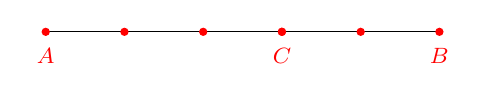
\begin{tikzpicture}[scale=1, font=\footnotesize, line join=round, line 
			cap=round, >=stealth]
			\path 
			(0,0) coordinate (A)
			(3,0) coordinate (C)
			(5,0) coordinate (B)
			;
			\draw (A)--(B);
			\foreach \x in {1,2,3,4}
			\fill[red] (\x,0) circle (1.5pt);
			\foreach \p/\r in {A/-90,B/-90,C/-90}
			\fill[red] (\p) circle (1.5pt) node[shift={(\r:3mm)}]{$\p$};
		\end{tikzpicture}
	\end{center}
	\choice
	{$\overrightarrow{AC}=\dfrac{3}{2}\overrightarrow{BC}$}
	{$\overrightarrow{AB}=\dfrac{5}{2}\overrightarrow{BC}$}
	{\True $\overrightarrow{AB}=\dfrac{5}{3}\overrightarrow{AC}$}
	{$\overrightarrow{CB}=\dfrac{2}{3}\overrightarrow{CA}$}
	\loigiai{
Vì 	$AB=\dfrac{5}{3}AC$ và $\overrightarrow{AB}, \overrightarrow{AC}$ cùng phương, cùng hướng. Suy ra $\overrightarrow{AB}=\dfrac{5}{3}\overrightarrow{AC}$.
}
\end{ex}

\begin{ex}%[10_HK1_LEQUYDON-NINHTHUAN_TL_TN]%[VU Ngoc Hao]%[0H2Y4-1]
	Cho hai véc-tơ $\vec{a},\vec{b}$ tùy ý. Tích vô hướng của hai véc-tơ $\vec{a},\vec{b}$ bằng
	\choice
	{$\overrightarrow{a}\cdot\overrightarrow{b}=\left| \overrightarrow{a} \right|\left| \overrightarrow{b} \right|$}
	{\True $\overrightarrow{a}\cdot\overrightarrow{b}=\left| \overrightarrow{a} \right|\left| \overrightarrow{b} \right|\cos \left( \overrightarrow{a},\overrightarrow{b} \right)$}
	{$\overrightarrow{a}\cdot\overrightarrow{b}=-\left| \overrightarrow{a} \right|\left| \overrightarrow{b} \right|$}
	{$\overrightarrow{a}\cdot\overrightarrow{b}=\left| \overrightarrow{a} \right|\left| \overrightarrow{b} \right|\sin \left( \overrightarrow{a},\overrightarrow{b} \right)$}
	\loigiai{
Cho hai vectơ $\vec{a}$	và $\vec{b}$ khác $\vec{0}$.Tích vô hướng của $\vec{a}$	và $\vec{b}$ là một số, được kí hiệu là $\vec{a}\cdot\vec{b}$ và xác định bởi công thức sau: $\overrightarrow{a}\cdot \overrightarrow{b}=\left| \overrightarrow{a} \right|\left| \overrightarrow{b} \right|\cos \left( \overrightarrow{a},\overrightarrow{b} \right)$.
}
\end{ex}

\begin{ex}%[10_HK1_LEQUYDON-NINHTHUAN_TL_TN]%[VU Ngoc Hao]%[0D3Y2-1]
	Với điều kiện nào của $m$ thì $f\left( x \right)=(m+1)x^2+mx+3$ là một tam thức bậc hai?
	\choice
	{$m=0$}
	{$m\ne 1$}
	{$m\ge -1$}
	{\True $m\ne -1$}
	\loigiai{
Để 	$f\left( x \right)=(m+1)x^2+mx+3$ là một tam thức bậc hai thì $m+1 \neq 0 \Leftrightarrow m\neq -1$.
}
\end{ex}

\begin{ex}%[10_HK1_LEQUYDON-NINHTHUAN_TL_TN]%[VU Ngoc Hao]%[0D3Y1-5]
\immini[thm]{	Cho hàm số $y=f\left( x \right)$ có tập xác định là $\left[-3;3 \right]$ và đồ thị của nó được biểu diễn bởi hình bên. Hàm số đồng biến trên khoảng nào sau đây?
	
	\choice
	{\True $(0;3)$}
	{$(-3;0)$}
	{$(-1;3)$}
	{$(-1;0)$}}{\begin{tikzpicture}[>=stealth,line join=round, line cap=round, scale=0.7]
		\draw[->] (-4,0)--(4,0) node[right]{$x$};
		\draw[->] (0,-2)--(0,5) node[below right]{$y$};
		\draw[fill] (3,0) circle (1.5pt) node[below]{$3$};
		\draw[fill] (-1,0) circle (1.5pt) node[below left]{$-1$};
		\draw[fill] (-3,0) circle (1.5pt) node[below left]{$-3$};
		\draw[fill] (0,-1) circle (1.5pt) node[right]{$-1$};
		\draw[fill] (0,1) circle (1.5pt) node[below right]{$1$};
		\draw[fill] (0,4) circle (1.5pt) node[left]{$4$};
		\fill (0,0) circle (1.5pt) node[below left]{$O$};
		\draw[dashed] (-3,0)--(-3,-1)--(0,-1) (3,0)--(3,4)--(0,4) (-1,0)--(-1,1);
		\draw[red,thick] (-3,-1)--(-1,1)--(0,1)--(3,4);
		
\end{tikzpicture}}
	\loigiai{
Từ đồ thị hàm số ta suy ra hàm số đồng biến trên khoảng $(-3;-1)$ và $(0;3)$. 
}
\end{ex}

\begin{ex}%[10_HK1_LEQUYDON-NINHTHUAN_TL_TN]%[VU Ngoc Hao]%[0D4Y2-1]
	Tập nghiệm của bất phương trình $x^2-x-6\le 0$ là
	\choice
	{$S=\left[-3;2 \right]$}
	{$S=\left( -\infty;-2 \right]\cup \left[3;+\infty \right)$}
	{$S=\left( -2;3 \right)$}
	{\True $S=\left[-2;3 \right]$}
	\loigiai{
	Đặt $f(x)=x^2-x-6$, ta có $a=1>0$ và $f(x)=0\Leftrightarrow \hoac{&x=3\\&x=-2.}$\\
Lập bảng xét dấu của $f(x)$ ta có
\begin{center}
	
\begin{tikzpicture}
		\tkzTabInit[nocadre=false, lgt=1.2, espcl=2.5]{$x$ /1,$f(x)$ /1}{$-\infty$,$-2$,$3$,$+\infty$}
		\tkzTabLine{,+,$0$,-,$0$,+,}
	\end{tikzpicture}
\end{center}
Dựa vào bảng xét dấu ta có tập nghiệm của bất phương trình là $S=\left[-2; 3 \right]$.	
}
\end{ex}

\begin{ex}%[10_HK1_LEQUYDON-NINHTHUAN_TL_TN]%[VU Ngoc Hao]%[0H1Y2-1]
	Cho tam giác $ABC$ có $AB=2a$, $\widehat{A}=30^{\circ}$, $\widehat{C}=45^{\circ}$. Độ dài cạnh $BC$ bằng
	\choice
	{$2a\sqrt{2}$}
	{$a\sqrt{3}$}
	{$\dfrac{a\sqrt{2}}{2}$}
	{\True $a\sqrt{2}$}
	\loigiai{
		\begin{center}
			\begin{tikzpicture}[scale=1, font=\footnotesize, line join=round, 
			line cap=round, >=stealth]
				\path 
				(4,0) coordinate (A)
				(-2,0) coordinate (B)
				(1.5,4) coordinate (C)
				;
				
				\draw (A)--(C)--(B);
				\draw (A)--(B) node[pos=0.5,below]{$2a$};
				\draw 	
				pic ["$30^\circ$",draw,angle radius=7mm]{angle=C--A--B}
				pic ["$45^\circ$",draw,angle radius=6mm]{angle=B--C--A};
				\foreach \p/\r in {A/-30,B/-150,C/90}
				\fill (\p) circle (1.5pt) node[shift={(\r:3mm)}]{$\p$};
			\end{tikzpicture}
		
	\end{center}
Áp dụng định lí $\sin$, ta có $\dfrac{AB}{\sin C}=\dfrac{BC}{\sin A} \Leftrightarrow BC = \dfrac{AB\cdot \sin A}{\sin C} =  \dfrac{2a\cdot  \sin 30^\circ}{\sin 45^\circ}=\dfrac{2a\cdot  \dfrac{1}{2} }{\dfrac{\sqrt{2}}{2}}=a\sqrt{2}$.	
}
\end{ex}

\begin{ex}%[10_HK1_LEQUYDON-NINHTHUAN_TL_TN]%[VU Ngoc Hao]%[0H2Y2-3]
	Cho $ABCD$ là hình bình hành tâm $O$. Khẳng định nào sau đây \textbf{sai}?
	\choice
	{\True $\overrightarrow{AB}+\overrightarrow{AC}=\overrightarrow{AD}$}
	{$\overrightarrow{AB}+\overrightarrow{AD}=\overrightarrow{AC}$}
	{$\overrightarrow{AB}+\overrightarrow{AD}=2\overrightarrow{AO}$}
	{$\overrightarrow{OA}+\overrightarrow{OB}+\overrightarrow{OC}+\overrightarrow{OD}=\overrightarrow{0}$}
	\loigiai{
		\begin{center}
			\begin{tikzpicture}[scale=1, font=\footnotesize, line join=round, 
			line cap=round, >=stealth]
				\path 
				(1,3) coordinate (A)
				(0,0) coordinate (B)
				(4,0) coordinate (C)
				($(A)+(C)-(B)$) coordinate (D)
				($(A)!0.5!(C)$) coordinate (O)
				;
				
				\draw (A)--(B)--(C)--(D)--cycle (A)--(C) (B)--(D);
				
				\foreach \p/\r in {A/90,B/-120,D/0,C/30,O/-90}
				\fill (\p) circle (1.5pt) node[shift={(\r:3mm)}]{$\p$};
			\end{tikzpicture}
			
			\end{center}
Theo quy tắc hình bình hành, ta có 	
$\overrightarrow{AB}+\overrightarrow{AD}=\overrightarrow{AC}=2\overrightarrow{AO} $ \\
 Do đó  khẳng định  	$\overrightarrow{AB}+\overrightarrow{AD}=\overrightarrow{AC}$; 
 $\overrightarrow{AB}+\overrightarrow{AD}=2\overrightarrow{AO}$ đúng.\\
Ta có $\overrightarrow{OA}$ và $\overrightarrow{OC}$; $\overrightarrow{OB}$ và 
$\overrightarrow{OD}$ là các cặp véc-tơ đối nhau.\\
 Suy ra 
 $\overrightarrow{OA}+\overrightarrow{OB}+\overrightarrow{OC}+\overrightarrow{OD}=
  \left( \overrightarrow{OA}+\overrightarrow{OC} \right) + \left( 
 \overrightarrow{OB}+\overrightarrow{OD} \right) = \overrightarrow{0} + 
 \overrightarrow{0} = \overrightarrow{0}$.\\
  Do đó  khẳng định $\overrightarrow{OA}+\overrightarrow{OB}+\overrightarrow{OC}+\overrightarrow{OD}=\overrightarrow{0}$ đúng. 
}
\end{ex}

\begin{ex}%[10_HK1_LEQUYDON-NINHTHUAN_TL_TN]%[VU Ngoc Hao]%[0D3Y1-2]
	Tập xác định của hàm số $y=\sqrt{x+2}-\sqrt{6-2x}$ là
	\choice
	{$\mathscr{D}=[2; 3]$}
	{$\mathscr{D}=[-3;-2]$}
	{\True $\mathscr{D}=[-2; 3]$}
	{$\mathscr{D}=[-3;2]$}
	\loigiai{
	Hàm số xác định khi và chỉ khi $\heva{&x+2\geq 0\\& 6-2x\geq 0} \Leftrightarrow \heva{&x\geq -2 \\ & x \leq 3}$ $\Leftrightarrow -2 \leq x \leq 3$.\\
Vậy tập xác định của hàm số là $\mathscr{D}=\left[ -2; 3 \right]$.	
}
\end{ex}

\begin{ex}%[10_HK1_LEQUYDON-NINHTHUAN_TL_TN]%[VU Ngoc Hao]%[0H1Y2-2]
	Cho tam giác $ABC$ có $BC=10,AC=8,\widehat{ACB}=30^{\circ}$. Diện tích tam giác $ABC$ bằng
	\choice
	{\True $20$}
	{$40$}
	{$20\sqrt{2}$}
	{$20\sqrt{3}$}
	\loigiai{
	\begin{center}
		\begin{tikzpicture}[scale=1, font=\footnotesize, line join=round, line 
		cap=round, >=stealth]
			\path 
			(1,3) coordinate (A)
			(0,0) coordinate (B)
			(4,0) coordinate (C)
			;
			
			\draw (A)--(B)--(C)--cycle;
			
			\foreach \p/\r in {A/90,B/-120,C/-60}
			\fill (\p) circle (1.5pt) node[shift={(\r:3mm)}]{$\p$};
		\end{tikzpicture}
	\end{center}
		
Ta có $S_{ABC}=\dfrac{1}{2}\cdot BC\cdot AC\cdot \sin C =\dfrac{1}{2}\cdot 10\cdot 8\cdot \sin 30^\circ = 20$.	
}
\end{ex}

\begin{ex}%[10_HK1_LEQUYDON-NINHTHUAN_TL_TN]%[VU Ngoc Hao]%[0D3B1-3]
	Cho hàm số $f\left( x \right)=\heva{&2x^2-3x+1\,\,\text{\text{ khi}}\,\,x<-1 \\&\sqrt{x+2}\,\,\text{\text{ khi}}\,\,x\ge -1}$. \\Giá trị của $P=f\left( -1 \right)+f\left( 2 \right)-3f\left( -2 \right)$ là
	\choice
	{$-35$}
	{$-25$}
	{\True $-42$}
	{$30$}
	\loigiai{
$f\left( -1 \right) = \sqrt{-1+2}=1$.\\
$f\left( 2 \right) = \sqrt{2+2}=\sqrt{4}=2$.\\	
$f\left( -2 \right) = 2\cdot \left( -2 \right) ^2 -3\cdot  \left( -2 \right) +1 = 15$.\\
Suy ra $P=f\left( -1 \right)+f\left( 2 \right)-3f\left( -2 \right) = 1 +2 -3\cdot 15 = -42$.
}
\end{ex}
\begin{ex}%[10_HK1_LEQUYDON-NINHTHUAN_TL_TN]%[VU Ngoc Hao]%[0H1G3-2]
		Từ một đỉnh tháp chiều cao $CD$, người ta nhìn hai điểm $A$ và $B$ trên mặt đất dưới các góc nhìn là $72^\circ 12'$ và $34^\circ 26'$. Ba điểm $A,B,D$ thẳng hàng. Tính chiều cao của tháp biết khoảng cách $AB=91$ m.
		\choice
		{\True $81{,}38$ m}
		{ $82{,}83$ m}
		{ $71{,}27$ m}
		{ $91{,}12$ m}	
	\begin{center}
		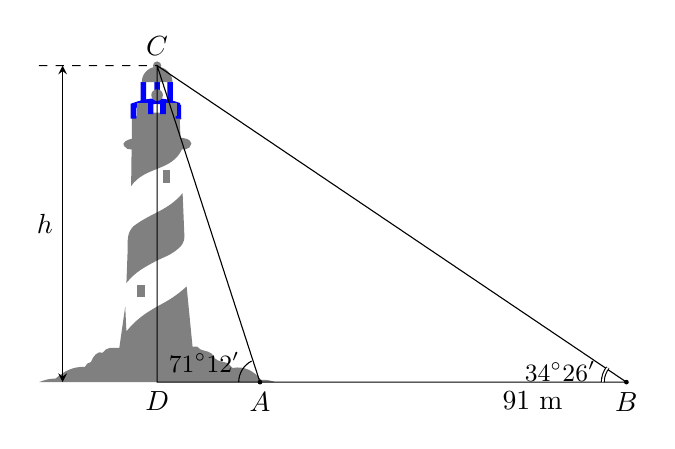
\begin{tikzpicture}[scale=.3,declare function={h=13.4;a=h/tan(72);b=h/tan(34);}]
			\fill[gray] (-5,0) 
			to[out=20,in=180] (-4.3,.15)
			to[out=40,in=180] (-3.05,.65)
			to[out=80,in=200] (-2.8,.85)
			to[out=70,in=160] (-2.3,1.25)
			to[out=50,in=190] (-2,1.45)
			--(-1.6,1.45)--(-1.35,3.2)--(-1.3,2.15)
			to[out=50,in=210] (0,3.2)
			to[out=28,in=222] (1.25,4.05)
			--(1.5,1.5)--(1.7,1.5)
			to[out=-40,in=180] (2,1.33)
			to[out=-10,in=110] (2.45,1)
			to[out=-40,in=160] (3,.8)
			to[out=-40,in=150] (3.2,.6)
			to[out=10,in=130] (4.4,.1)
			to[out=0,in=160] (5,0)
			--cycle;
			\fill[gray] (-.85,3.6) rectangle (-.53,4.1);
			\fill[gray] (-1.3,4.2)
			to[out=50,in=208] (0,5.15)
			to[out=25,in=225] (1,5.75)
			to[out=50,in=275] (1.15,6.3)
			--(1.08,8)
			to[out=-130,in=37] (-1,6.6)
			to[out=-135,in=88] (-1.25,5.5)
			--cycle;
			\fill[gray] (.25,8.45) rectangle (.55,9);
			\fill[gray] (-1.1,8.3)
			to[out=55,in=245] (1.05,9.85)--(1.2,9.85)
			to[out=10,in=263] (1.45,10.1)
			to[out=100,in=-10] (.99,10.35)--(.96,11.1)--(1.05,11.15)
			to[out=155,in=20] (-1.07,11.2)--(-1.07,10.3)
			to[out=-175,in=135] (-1.4,10)
			to[out=-55,in=190] (-1.08,9.85)--cycle;
			\draw[blue,line width= 2pt] 
			(.9,11.15)--(.9,11.75)
			(.25,11.35)--(.25,11.9)
			(-.28,11.35)--(-.28,11.9)
			(-1,11.15)--(-1,11.7)
			to[out=20,in=160] (0.94,11.7)
			(.55,11.8)--(.55,12.7)
			(-.58,11.8)--(-.58,12.7)
			(0,11.9)--(0,12.7);
			\draw[gray,line width=4pt] 
			(.6,11.25)--(.6,11.8)
			(-.63,11.25)--(-.63,11.8);
			\fill[gray] (0,12.15) circle (7pt)
			(.65,12.7) arc (0:180:.65) -- cycle
			(0,13.4) circle (5pt);
			\path 
			(0,0) coordinate (C)node[below]{$D$}
			(a,0) coordinate (A)
			(b,0) coordinate (B)
			(0,h) coordinate (D)node[above]{$C$};
			\foreach \i/\g in { A/-90, B/-90} \fill (\i)circle(.1) node[shift={(\g:.25)}] {$\i$};
			\draw (C)--(B)node[pos=.8, below]{$91$ m}--(D)--cycle (A)--(D)
			(A)+(-.9,0) arc (180:117:1)node[pos=.9, left]{\small $71^\circ 12'$};
			\draw[double] (B)+(-1,0) arc (180:142:1)node[pos=.7, left]{\small $34^\circ 26'$};
			\draw[dashed] (-5,h)--(D);
			\draw[stealth-stealth] (-4,0) -- (-4,h)node[pos=.5, left]{$h$};
		\end{tikzpicture}
	\end{center}
	\loigiai{
		Vì tam giác $\Delta DAC$ vuông tại $D$ nên $\widehat{ACD} = 90^\circ - \widehat{DAC}= 90^\circ - 71^\circ12'= 18^\circ48'$.\\
		Vì tam giác $\Delta DBC$ vuông tại $D$ nên $\widehat{BCD} = 90^\circ - \widehat{DBC}= 90^\circ - 34^\circ26'= 55^\circ34'$.\\
		Áp dụng định lí $\sin$ cho tam giác $\Delta DAC$ ta được:
		$\dfrac{CD}{\sin \widehat{DAC}}=\dfrac{DA}{\sin \widehat{ACD}} \Leftrightarrow DA =\dfrac{CD.\sin \widehat{ACD}}{\sin \widehat{DAC}}$.\\
		Áp dụng định lí $\sin$ cho tam giác $\Delta DBC$ ta được:
		$\dfrac{CD}{\sin \widehat{DBC}}=\dfrac{DB}{\sin \widehat{DCB}} \Leftrightarrow DB =\dfrac{CD\cdot\sin \widehat{DCB}}{\sin \widehat{DBC}}$.\\
		Ta có:\\
		$$
		\begin{aligned}
			 DB- DA =AB & \Leftrightarrow  CD. \left( \dfrac{\sin \widehat{DCB}}{\sin \widehat{DBC}} - \dfrac{\sin \widehat{ACD}}{\sin \widehat{DAC}} \right) = AB  \\
			& \Leftrightarrow CD= \dfrac{AB}{  \dfrac{\sin \widehat{DCB}}{\sin \widehat{DBC}} - \dfrac{\sin \widehat{ACD}}{\sin \widehat{DAC}} } = \dfrac{91}{  \dfrac{\sin 55^\circ34'}{\sin 34^\circ26'} - \dfrac{\sin 18^\circ48'}{\sin 71^\circ12'} }  \approx 81{,}38\, \mathrm{(m)}.
		\end{aligned}
		$$
	Vậy chiều cao của tháp khoảng $81{,}38 $ (m).
		
		}
\end{ex}

\begin{ex}%[10_HK1_LEQUYDON-NINHTHUAN_TL_TN]%[VU Ngoc Hao]%[0H2K4-1]
	Cho tam giác $ABC$ vuông tại $A$ có $AB=a,AC=a\sqrt{3}$, gọi $H$ là chân đường cao hạ từ $A$. Tích vô hướng của $\overrightarrow{BH}\cdot\overrightarrow{AC}$ bằng
	\choice
	{$\dfrac{a^2}{4}$}
	{$\dfrac{\sqrt{3}a^2}{4}$}
	{$\dfrac{3a^2}{2}$}
	{\True $\dfrac{3a^2}{4}$}
	\loigiai{
		\begin{center}
			\begin{tikzpicture}
				\coordinate (A) at (0,0);
				\coordinate (B) at (-1,-2);
				\coordinate (C) at (3,-2);
				\draw (A)node[above]{$A$}--(B)node[left]{$B$}--(C)node[right]{$C$}--cycle;
				\coordinate (H) at (0,-2);
				\draw [dashed] (A)--(H);
				\draw 	
				pic [draw,angle radius=2mm]{right angle=B--A--C}
				pic [draw,angle radius=2mm]{right angle=C--H--A};
				\draw (H) node[below]{$H$};
			\end{tikzpicture}
		\end{center}
Trong tam giác $\Delta ABC$ vuông tại $A$, ta có $\tan{\widehat {B}}=\dfrac{AC}{AB} = \dfrac{a\sqrt{3}}{a}=\sqrt{3} \Rightarrow \widehat {B} = 60^\circ$.\\
Trong tam giác $\Delta ABH$ vuông tại $H$, ta có $\cos{\widehat{B}} = \dfrac{HB}{AB}\Rightarrow BH = AB\cdot \cos{\widehat{B}} = a\cdot\cos{60^\circ} = \dfrac{a}{2}$.\\
Lại có $\left( \vec{BH};\vec{AC} \right) = 30^\circ$. Suy ra $\overrightarrow{BH}\cdot\overrightarrow{AC} = BH\cdot AC\cdot\cos{\left(\vec{BH};\vec{AC} \right)} = \dfrac{a}{2} \cdot a\sqrt{3}\cdot
\cos{30^\circ}=\dfrac{3a^2}{4}$.

}
\end{ex}

\begin{ex}%[10_HK1_LEQUYDON-NINHTHUAN_TL_TN]%[VU Ngoc Hao]%[0D4K2-1]
	Cho tam thức bậc hai $f(x)=2x^2+bx+c$ biết $f(x)>0\Leftrightarrow x\in (-\infty;x_1)\cup (x_2;+\infty )$ và $\left| x_1-x_2 \right|=\dfrac{3}{2}$. Khi đó giá trị của biểu thức $b^2-8c$ bằng
	\choice
	{$8$}
	{$10$}
	{\True $9$}
	{$11$}
	\loigiai{
Theo đề bài ta có $x_1, x_2$ là hai nghiệm của tam thức bậc hai $f(x)=2x^2+bx+c$.\\
Áp dụng định lí Vi-ét, ta được: $\heva{&x_1 +x_2 =-\dfrac{b}{a}\\& x_1\cdot x_2 = \dfrac{c}{a}}.$\\
Ta có	
	$$
\begin{aligned}
& \left| x_1-x_2 \right|=\dfrac{3}{2}\\
 \Leftrightarrow &  \left( x_1-x_2 \right)^2=\dfrac{9}{4}  \\
 \Leftrightarrow & \left( x_1+x_2 \right)^2 -4x_1.x_2=\dfrac{9}{4}\\
 \Leftrightarrow & \dfrac{b^2}{4} -4\cdot\dfrac{c}{2} =\dfrac{9}{4}\\
 \Leftrightarrow & \dfrac{b^2 -8c}{4} =\dfrac{9}{4}\\
 \Leftrightarrow & b^2 -8c =9.
\end{aligned}
$$
}
\end{ex}

\begin{ex}%[10_HK1_LEQUYDON-NINHTHUAN_TL_TN]%[VU Ngoc Hao]%[0D3K2-1]
	Cho hàm số $y=ax^2+bx+c (a\ne 0)$ có đồ thị là parabol $(P)$. Biết đồ thị của hàm số đi qua điểm $A(0;3)$ và có đỉnh $I(1;1)$. Tính tổng $S=a^2+b^2+c^2$.
	\choice
	{$4$}
	{$25$}
	{$20$}
	{\True $29$}
	\loigiai{
Vì đồ thị hàm số đi qua điểm $A(0;3)$ nên ta có: $a\cdot 0^2 +b\cdot0 +c =3 \Leftrightarrow c=3$.\\
Vì $(P)$ có đỉnh $I(1;1)$ nên $\heva{&-\dfrac{b}{2a}=1\\&-\dfrac{\Delta}{4a}=1} \Leftrightarrow \heva{&b=-2a\\&b^2-12a=-4a}$\\
$\Leftrightarrow \heva{&b=-2a\\&b^2-8a=0} \Leftrightarrow \heva{&b=-2a\\&4a^2-8a=0} \Rightarrow \heva{&a=2\\&b=-2\cdot 2=-4.}$\\
Vậy $S=a^2+b^2+c^2 =2^2 + \left( -4 \right)^2 +3^2 =29$.	
}
\end{ex}

\begin{ex}%[10_HK1_LEQUYDON-NINHTHUAN_TL_TN]%[VU Ngoc Hao]%[0H2B3-5]
	Cho $ABCD$ là hình bình hành tâm $O$. Gọi $M$ là trung điểm của $OD$. Khẳng định nào sau đây đúng?
	\choice
	{$\overrightarrow{AM}=\dfrac{1}{3}\overrightarrow{AB}+\dfrac{1}{2}\overrightarrow{AD}$}
	{\True $\overrightarrow{AM}=\dfrac{1}{4}\overrightarrow{AB}+\dfrac{3}{4}\overrightarrow{AD}$}
	{$\overrightarrow{AM}=\dfrac{1}{3}\overrightarrow{AB}+\dfrac{1}{2}\overrightarrow{AD}$}
	{$\overrightarrow{AM}=-\dfrac{1}{8}\overrightarrow{AB}+\dfrac{3}{8}\overrightarrow{AD}$}
	\loigiai{
		\begin{center}
			\begin{tikzpicture}[scale=1, font=\footnotesize, line join=round, 
				line cap=round, >=stealth]
				\path 
				(1,3) coordinate (A)
				(0,0) coordinate (B)
				(4,0) coordinate (C)
				($(A)+(C)-(B)$) coordinate (D)
				($(A)!0.5!(C)$) coordinate (O)
				($(O)!0.5!(D)$) coordinate (M)
				;
				
				\draw (A)--(B)--(C)--(D)--cycle (M)--(A)--(C) (B)--(D);
				
				\foreach \p/\r in {A/90,B/-120,D/0,C/30,O/-90,M/-90}
				\fill (\p) circle (1.5pt) node[shift={(\r:3mm)}]{$\p$};
			\end{tikzpicture}
			
		\end{center}
Vì $O$ là trung điểm của $BD$ nên $\vec{AO}=\dfrac{1}{2}\left( \vec{AD} +\vec{AB} \right)$.\\			
Vì $M$ là trung điểm của $OD$ nên \\
$$\vec{AM} =\dfrac{1}{2} \left( \vec{AD} 
	+\vec{AO} \right) =\dfrac{1}{2}\vec{AD} +  \dfrac{1}{2}\vec{AO} = 
	\dfrac{1}{2}\vec{AD}+\dfrac{1}{2} \cdot \dfrac{1}{2} \left( \vec{AD} +\vec{AB} \right)$$\\
	$$ 
	 =  \dfrac{1}{2}\vec{AD} +\dfrac{1}{4}\vec{AD} +\dfrac{1}{4}\vec{AB}=\dfrac{1}{4}\vec{AB} +\dfrac{3}{4}\vec{AD}.  
$$

}
	
\end{ex}


\Closesolutionfile{ans}
%\begin{center}
%	\textbf{ĐÁP ÁN}
%	\inputansbox{10}{ans/ans}	
%\end{center}
\begin{center}
	\textbf{PHẦN 2 - TỰ LUẬN}
\end{center}



\begin{bt}%[0H2Y2-3]%[0H1B2-1]%[0H1B2-2]
	Cho tam giác $ABC$ có $AB=3a,AC=4a,\widehat{BAC}=60^{\circ}$. Gọi $M$ là trung điểm của $BC$ và $I$ là trung điểm của $AM$.
	\begin{enumerate}
		\item Chứng minh rằng: $2\overrightarrow{IA}+\overrightarrow{IB}+\overrightarrow{IC}=\overrightarrow{0}$.
		\item Tính cạnh $BC$, diện tích tam giác $ABC$ và độ dài đường cao $AH$ của tam giác $ABC$.
		\item Tính tích vô hướng $\overrightarrow{BA}\cdot\overrightarrow{CB}$.
	\end{enumerate}
	\loigiai{
		\begin{center}
			\begin{tikzpicture}[scale=1, font=\footnotesize, line join=round, 
			line cap=round, >=stealth]
				\path 
				(1,3) coordinate (A)
				(0,0) coordinate (B)
				(4,0) coordinate (C)
				($(B)!0.5!(C)$) coordinate (M)
				($(A)!0.5!(M)$) coordinate (I)
				($(B)!(A)!(C)$) coordinate (H)
				;
				
				\draw (A)--(B)--(C)--cycle (H)--(A)--(M);
				\draw pic [draw,angle radius=2mm]{right angle=C--H--A};
				\foreach \p/\r in {A/90,B/-120,C/-60,M/-90,I/0,H/-90}
				\fill (\p) circle (1.5pt) node[shift={(\r:3mm)}]{$\p$};
			\end{tikzpicture}
		\end{center}
		\begin{enumerate}
		\item
		Vì $M$ là trung điểm của $BC$ nên $\overrightarrow{IB} + \overrightarrow{IC} =2\overrightarrow{IM}$.\\
		Vì $I$ là trung điểm của $AM$ nên $\overrightarrow{IA} +\overrightarrow{IM}=\overrightarrow{0}$.\\
		Ta có 
		 $2\overrightarrow{IA}+\overrightarrow{IB}+\overrightarrow{IC}=2\overrightarrow{IA} + 2\overrightarrow{IM} = 2 \left( \overrightarrow{IA} + \overrightarrow{IM} \right) =2\cdot\overrightarrow{0}= \overrightarrow{0} $.
		\item $BC^2=AB^2 +AC^2 -2\cdot AB\cdot AC\cdot \cos{\widehat{BAC}}=9a^2 +16a^2 -2\cdot 3a\cdot 4a\cdot \cos{60^\circ}=13a^2$\\
		$ \Rightarrow BC= a\sqrt{13}$. \\
		Diện tích tam giác $ABC$: $S_{\triangle ABC}= \dfrac{1}{2}\cdot AB\cdot AC\cdot \sin{\widehat{BAC}}=\dfrac{1}{2}\cdot 3a\cdot 4a\cdot \sin{60^\circ}=3\sqrt{3}a^2$. \\
		Ta có $S_{\triangle ABC}= \dfrac{1}{2}\cdot AH\cdot BC \Rightarrow AH=\dfrac{2S_{\triangle ABC}}{BC}=\dfrac{2\cdot 3\sqrt{3}a^2}{a\sqrt{13}
		}=\dfrac{6a\sqrt{39}}{13}$.
		\item 
		Áp dụng định lí cô-sin trong tam giác $ABC$, ta được:
		$$\cos \widehat{ABC} =\dfrac{BA^2 +BC^2 -AC^2}{2\cdot BA\cdot BC} =\dfrac{9a^2 +13a^2-16a^2}{2\cdot 3a\cdot a\sqrt{13}}=\dfrac{1}{\sqrt{13}}.$$\\
		Ta có $\widehat{\left( \overrightarrow{BA}, \overrightarrow{CB} \right)} =180^\circ -\widehat{ABC}$.\\
		Do đó $\cos{\left( \widehat{\left( \overrightarrow{BA}, \overrightarrow{CB} \right)}\right)}=\cos{\left(  180^\circ -\widehat{ABC}\right)}=-\cos{\widehat{ABC}}=-\dfrac{1}{\sqrt{13}}$.\\
		Suy ra
		$\overrightarrow{BA}\cdot\overrightarrow{CB}=BA\cdot CB\cdot  \cos{\left( \widehat{\left( \overrightarrow{BA}, \overrightarrow{CB} \right)}\right)}=3a\cdot a\sqrt{13}\cdot \left(-\dfrac{1}{\sqrt{13}}\right)=-3a^2$.
	\end{enumerate}


}
\end{bt}
\begin{bt}%[0D3B2-3]
	Vẽ đồ thị hàm số bậc hai $y=x^2-2x-3$.
	\loigiai{
		\immini{Ta có $\Delta=(-2)^2-4\cdot1\cdot(-3)=16$.
			\begin{itemize}
				\item Tọa độ đỉnh $I(1;-4)$.
				\item Trục đối xứng $x=1$.
				\item Giao điểm của parabol với trục tung là $A(0;-3)$.
				\item Giao điểm của parabol với trục hoành là $B(-1;0)$ và $C(3;0)$.
				\item Điểm đối xứng với điểm $A(0;-3)$ qua trục đối xứng $x=1$ là $D(2;-3)$.
			\end{itemize}
			Vẽ parabol đi qua các điểm được xác định ở trên, ta nhận được đồ thị hàm số $y=x^2-2x-3$.
		}{
			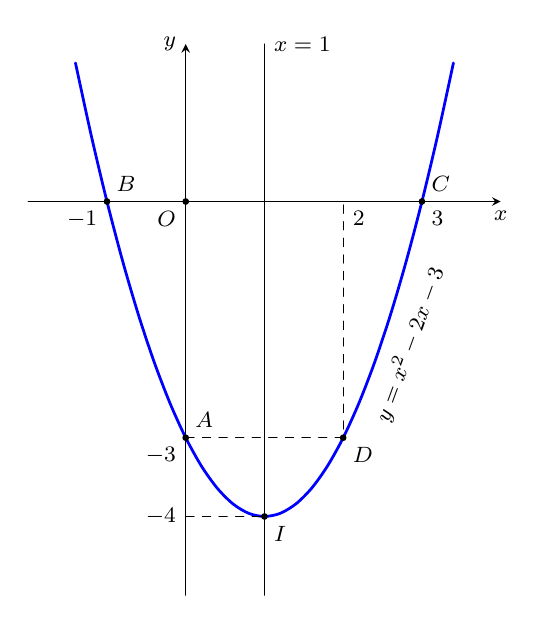
\begin{tikzpicture}[scale=1, font=\footnotesize, line join=round, line cap=round, >=stealth]
				\draw[->](-2,0)--(0,0)node[below left]{$O$}--(4,0)node[below]{$x$};
				\draw[->](0,-5)--(0,2)node[left]{$y$};
				\draw[smooth,blue, line width=1]
				plot[domain=-1.4:3.4](\x,{(\x)^2-2*(\x)-3})
				;
				\draw[fill](-1,0)circle(1pt)node[below left]{$-1$}node[above right]{$B$};
				\draw[fill](3,0)circle(1pt)node[below right]{$3$}node[above right]{$C$};
				\draw[fill](0,-3)circle(1pt)node[below left]{$-3$}node[above right]{$A$};
				\draw[dashed](0,-4)node[left]{$-4$}--(1,-4)node[below right]{$I$};
				\draw(1,-5)--(1,2)node[right]{$x=1$};
				\draw[dashed](0,-3)--(2,-3)node[below right]{$D$}--(2,0)node[below right]{$2$};
				\draw(2.7,-3)node[above right,rotate=70]{$y=x^2-2x-3$};
				\draw[fill](0,0)circle(1pt);
				\draw[fill](1,-4)circle(1pt);
				\draw[fill](2,-3)circle(1pt);
		\end{tikzpicture}}
	}
\end{bt}

\begin{bt}%[0D4K2-2]
	Tìm các giá trị của tham số $m$ để bất phương trình $x^2-2(m+1)x+5m-1<0$ vô nghiệm.
	\loigiai{Ta có $f(x)=x^2-2(m+1)x+5m-1<0$ vô nghiệm \\$\Leftrightarrow f(x)=x^2-2(m+1)x+5m-1 \geq 0 \,\,\forall x\in \mathbb{R}$\\
	$\Leftrightarrow \Delta' =m^2 -3m +2 \leq 0$\\
	$\Leftrightarrow 1\leq m\leq 2$.	\\
	Vậy $m \in [1;2]$ thì bất phương trình đã cho vô nghiệm.
	}
\end{bt}

\begin{bt}%[0D3K2-5]
	Một vận động viên bóng chuyền đánh bóng qua lưới, biết quỹ đạo chuyển động của bóng là một cung parabol $(P)$ được mô phỏng bởi phương trình $h(t)=-0{,}4t^2+2t+0{,}4$, trong đó $h$ là chiều cao của bóng tính bằng mét và $t$ là thời gian bóng di chuyển tính bằng giây.
	\begin{enumerate}
		\item Tìm thời gian để bóng đạt độ cao lớn nhất.
		\item Tìm khoảng thời gian mà bóng cao hơn lưới, biết rằng chiều cao của lưới bằng $2{,}4$ m.
	\end{enumerate}

\definecolor{battleshipgrey}{rgb}{0.52, 0.52, 0.51}

\begin{tikzpicture}[line join=round, line cap=round,scale=1.7,transform shape]
	\clip (-4,-2.5) rectangle (5,2.5);
		
	\tikzset{vdv/.pic={
			\def\T{ 
				(-.4,1.55)
				..controls +(175:.3) and +(95:.4) ..  (-.8,1.1)--(-.76,1.12)--(-.77,1.06)--(-.7,1.08)--(-.72,1.02)--(-.62,1.06)
				..controls +(-15:.15) and +(45:.15) ..  (-.64,.92)
				..controls +(175:.1) and +(-155:.05) ..  (-.8,.85)
				..controls +(155:.05) and +(15:.05) .. (-1.05,.9)
				..controls +(75:.1) and +(-85:.05) .. (-1.02,1.3)
				..controls +(45:.1) and +(-145:.05) .. (-.9,1.5)
				..controls +(75:.15) and +(35:0) .. (-.97,1.48)
				..controls +(165:.1) and +(-90:0) .. (-1.02,1.7)
				..controls +(145:.07) and +(75:0) .. (-1.07,1.55)
				..controls +(115:.05) and +(-85:0) .. (-1.09,1.74)
				..controls +(145:.07) and +(-90:0) .. (-1.12,1.54)
				..controls +(115:.05) and +(-85:0) .. (-1.16,1.69)
				..controls +(145:.07) and +(-90:0) .. (-1.17,1.53)
				..controls +(135:.05) and +(-85:0) .. (-1.26,1.6)
				..controls +(-145:.08) and +(90:.3) .. (-1.16,1.3)
				..controls +(-95:.08) and +(90:.3) .. (-1.25,.8)
				..controls +(-25:.05) and +(175:.25) .. (-.8,.62)
				..controls +(-40:.5) and +(85:.15) .. (-.65,-.18)--(-.62,-.18)
				..controls +(-120:.5) and +(50:.2) .. (-.75,-1.2)
				..controls +(-130:.5) and +(50:.25) .. (-.95,-2)
				..controls +(-130:.1) and +(150:.3) .. (-.82,-2.3)
				..controls +(-60:.1) and +(-40:.5) .. (-.72,-2.1)
				..controls +(70:.1) and +(-40:.1) .. (-.76,-1.98)
				..controls +(90:.4) and +(-70:.2) .. (-.46,-1.16)--(-.26,-.65)
				..controls +(-50:.4) and +(120:.4) .. (.3,-1.23)
				..controls +(-95:.5) and +(85:.4) .. (.4,-2)
				..controls +(-115:.3) and +(165:.2) .. (.65,-2.26)
				..controls +(-20:.4) and +(-10:.25) .. (.7,-2.1)--(.74,-2.05)--(.6,-1.94)
				..controls +(120:.2) and +(-10:.2) .. (.5,-1)
				..controls +(110:.45) and +(-120:0.15) .. (.05,-.14)--(.1,-.12)
				..controls +(110:.3) and +(-70:0.15) .. (0,.8)
				..controls +(70:.05) and +(-170:0.05) .. (.1,.9)
				..controls +(25:.7) and +(-170:0.5) .. (1.2,1.7)
				..controls +(70:.1) and +(-20:0.1) .. (.92,1.74)
				..controls +(120:.05) and +(-120:0.05) .. (.98,1.8)
				..controls +(120:.05) and +(70:0.2) .. (.76,1.6)
				..controls +(-120:.05) and +(55:0.25) .. (.35,1.25)
				..controls +(170:.05) and +(-5:0.25) .. (-.1,1.12)
				..controls +(-170:.02) and +(45:0.05) .. (-.2,1.02)--(-.28,1.04)--(-.29,1.1)
				..controls +(20:.15) and +(-130:0.08) .. (-.23,1.35)
				..controls +(160:.17) and +(-45:0.25) .. cycle
				;}
			\draw \T;
			\fill \T;
	}}
	
	
	\draw (-3,-1)--(5,-1);
	
	\draw[fill=blue] (-1.55,.86) circle (3pt);
	\draw[fill=blue] (4.7,-.875) circle (3pt);
	
	\node at (0,0) [right]{\tiny $2{,}4$ m};
	\draw[line width=4] (0,.43)--(0,-1);
	\draw[line width=2] (0,.43)--(0,1);
	\draw[<->] (0.1,1)--(0.1,-1);
	%\draw[fill=black] (-2.5,.02) circle (.3pt);
	%\node[fill=black,rectangle,draw] (.2) at (-2.2,-.5) {};
	\draw[->] (-1.5,1)..controls +(40:1.5) and +(135:3) ..  (4.6,-.68);
	\path (-2,0)pic[scale=.40, fill=red ]{vdv}
	;
	
\end{tikzpicture}
	\loigiai{
	\begin{enumerate}
		\item Thời gian để bóng đạt độ cao lớn nhất là $t=-\dfrac{b}{2 a}=-\dfrac{2}{-0{,}4\cdot2}=2{,}5$ (s).
		\item Khoảng thời gian mà bóng cao hơn lưới là
		$$
		\begin{aligned}
			& -0{,}4 t^2+2 t+0{,}4>2,4 \Leftrightarrow 0{,}4-2 t+2<0 \\
			& \Leftrightarrow 1{,}38 \approx \dfrac{5-\sqrt{5}}{2}<t<\frac{5+\sqrt{5}}{2} \approx 3{,}62.
		\end{aligned}
		$$
	\end{enumerate}

}
\end{bt}





